\documentclass[12pt]{article}
%\usepackage{stdheadstart}
\usepackage{xargs}
\usepackage{physics}
\usepackage{tikz}
\usepackage{amsmath,amssymb}
\usepackage{hyperref}
%\insheadstart{images/}


\begin{document}

	\title{Symmetry suppression of allowed transitions between energy eigenstates of a Hamiltonian perturbed from a high symmetry.}	
	\maketitle
	
	\abstract{It has been observed in quantum dots with $C_{3v}$ symmetry that certain electronic transitions allowed by the dipole approximation selection rule are unresolvable in the measured photoluminiscence (PL) spectrum. We provide a theoretical model that predicts these spectral lines to be severely weakened if the Hamiltonian is considered to be perturbed from one with a higher spatial symmetry. An expression for the suppressing factor of the spectral line intensity is given in 1st order perturbation theory.}
	
	\section{Introduction}
	Karlsson et al \cite{karlsson} have studied the PL spectrum of InGaAs $C_{3v}$-symmetric quantum dots (QDs). Their model assumes that the QD-Hamiltonian eigenstates which interact with electromagnetic waves on the studied interval of the spectrum are given by considering the symmetry breaking of exciton complex fine structure, which splits total angular momentum $J$ eigenstates into energy levels which transform as double group irreps. By using rudimentary group theory, the energy levels, their degeneracies, and their allowed transitions can be calculated for all excitonic complexes, as was done by this particular QD. However, it was found that the number of spectral lines resolvable in a spectral feature associated with a specific excitonic transition is smaller than the predicted number for several exciton complex transitions, namely $X_{10}\to vac., 2X_{20}\to X_{10},2X_{11}\to X_{10}, 2X_{11}\to X_{01}, 2X^+_{21}\to X^+_{11}$. Since the number of allowed transitions lowers if the Hamiltonian is altered to commute with more rotations (e.g. to $D_{3h}$ or $C_{6v}$ point group symmetry), the effect was dubbed "symmetry elevation". However, no explanation for why symmetry elevation occurs was found.
	
	What the previous work on symmetry elevation in QDs did not consider is the nanocrystallic lattice that constitutes the QDs inside the potential well. The InGaAs QDs are formed by a lattice which does possess a 6-fold rotation along the $z$-axis. Even though the full Hamiltonian still only possesses $C_{3v}$ symmetry, since it is ultimately dominated by the lower-symmetry potential well boundary shape, it can be modelled as a high-symmetry Hamiltonian which underwent symmetry breaking with a small perturbation and enjoys certain approximate symmetries, which still turn out to have a considerate effect in 1st order expansion. To obtain a theoretical description of the effects of these approximate symmetries, we first consider 1st order perturbation theory and describe a surjective mapping of basis vectors of irreps of the larger point group onto the basis vectors of irreps of its point subgroup, which allows us to determine the mapping of high-symmetry Hamiltonian eigenstates onto the low-symmetry Hamiltonian eigenstates under symmetry breaking, and then we emply Fermi's golden rule to quantify the suppression of certain spectral lines. The manifestation of de-intensifying of specific spectral lines due to approximate symmetries will be named "symmetry suppression".
	
	\section{Theoretical model of symmetry suppression}
	We shall first outline a general approach to describing a non-specific minimally symmetry-broken Hamiltonian, and then argue for why the assumptions made are justified in the case of InGaAs QDs. 
	\subsection{Symmetry breaking as basis vector surjection}
	
	The theoretical model derived in \ref{sec:perturbation} considers the perturbation of a degenerate energy level under symmetry breaking. In general, the energy level split into multiple energy levels with lower degeneracies. This process is described theoretically in \cite{dresselhaus} like so: every energy level of a Hamiltonian $\hat{H}$ equipped with a symmetry group $G$ transforms according to a specific irrep $\Gamma^{(G)}$ of $G$ (when disregarding accidental degeneracy). Under symmetry breaking, the new symmetry group $G_-$ is a subgroup of $G$, and $\Gamma^{(G)}$ is in general a reducible representation of $G_-$. Reducing it yields a set of irreps of $G_-$, each of which corresponds to a split-off energy level of the perturbed Hamiltonian.
	
	In our theoretical moment, we shall wish to calculate the overlap integrals between a perturbed eigenstate and a chosen basis of the degenerate energy level it perturbed from. We can lower the amount of integrals needed to be calculated by considering the orthonormal basis of the high-symmetry group irrep $\Gamma^{(G)}$. If this irrep is reducible into multiple irreps in $G_-$,, there exists a similarity transform of $\Gamma^{(G)}$ which brings it into a block-diagonal form for all elements in $G_-$. Then the set of its basis vectors can be partitioned into multiple subsets which transform according to different irreps of $G_-$, and therefore correspond to different energy levels in the perturbed Hamiltonian. Identifying the perturbed energy level identifies the partitioned subset, and an eigenvector in the perturbed energy level must be orthogonal to all the basis vectors of $\Gamma^{(G)}$ outside of that subset.
	
	This partitioning can be described by a function which maps every basis vector of all irreps of $G$ onto a basis vector of $G_-$. The multiplication table of $G_-$ is obtained by removing rows and columns from the multiplication table of $G$, hence the regular representation of $G$ contains the regular representation of $G_-$ and therefore also every irrep of $G_-$. Since then for every irrep of $G_-$ there exists an irrep of $G$ which contains it, the function describing basis vector partitioning is surjective, but as the number of basis vectors lowers with the group order, it is non-injective. This function will be referred to as the basis vector surjection. To calculate it, we do not need to find the correct similarity transforms, since the blocks in the block diagonal must have the same traces as the traces of the irreps they map onto, and so the correct partitioning can be determined by checking these subtraces for one element in each conjugacy class.
	
	\begin{figure}[h]
	\begin{center}
	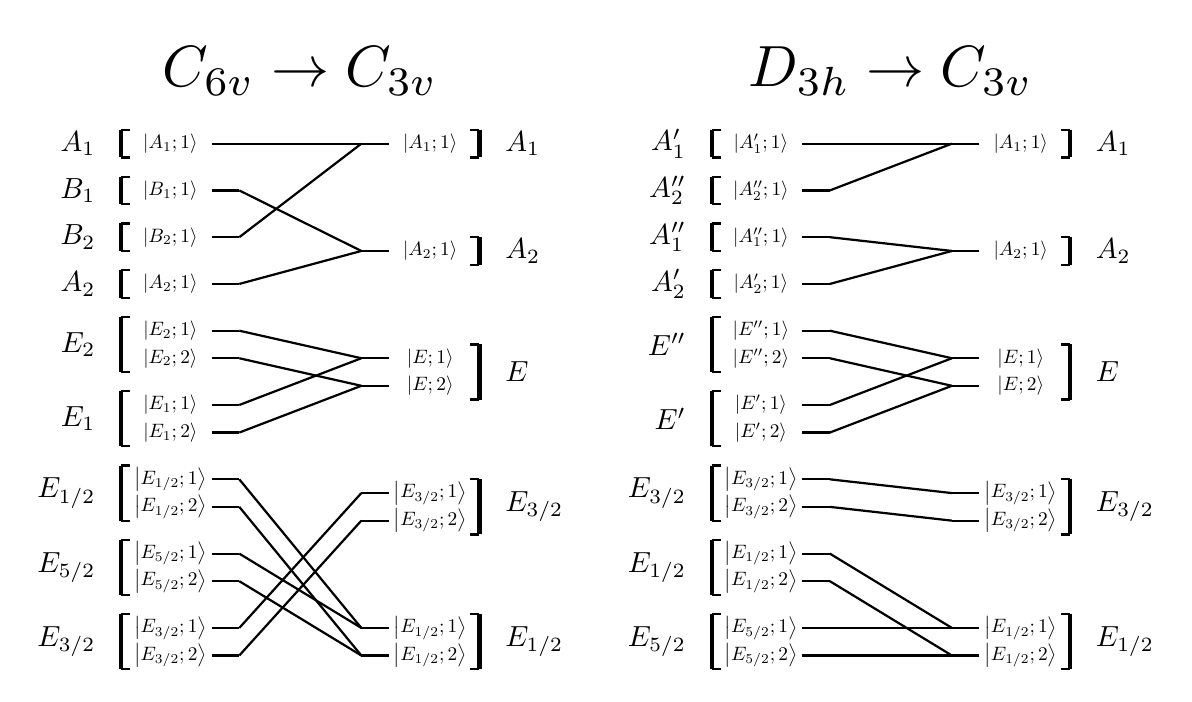
\begin{tikzpicture}[scale=0.5]
\draw[thick] (0,0) -- (0.7,0) node[pos=-1.5,scale=0.7] {$\ket{A_1;1}$};
\draw[ultra thick] (-2.3,0.35) -- (-2.3,-0.35) node[pos=0.5,left=5pt,scale=1.0499999999999998] {$A_1$};
\draw[thick] (-2.3,0.35) -- (-2.07,0.35);
\draw[thick] (-2.3,-0.35) -- (-2.07,-0.35);
\draw[thick] (0,-1.1875) -- (0.7,-1.1875) node[pos=-1.5,scale=0.7] {$\ket{B_1;1}$};
\draw[ultra thick] (-2.3,-0.8375) -- (-2.3,-1.5375) node[pos=0.5,left=5pt,scale=1.0499999999999998] {$B_1$};
\draw[thick] (-2.3,-0.8375) -- (-2.07,-0.8375);
\draw[thick] (-2.3,-1.5375) -- (-2.07,-1.5375);
\draw[thick] (0,-2.375) -- (0.7,-2.375) node[pos=-1.5,scale=0.7] {$\ket{B_2;1}$};
\draw[ultra thick] (-2.3,-2.025) -- (-2.3,-2.725) node[pos=0.5,left=5pt,scale=1.0499999999999998] {$B_2$};
\draw[thick] (-2.3,-2.025) -- (-2.07,-2.025);
\draw[thick] (-2.3,-2.725) -- (-2.07,-2.725);
\draw[thick] (0,-3.5625) -- (0.7,-3.5625) node[pos=-1.5,scale=0.7] {$\ket{A_2;1}$};
\draw[ultra thick] (-2.3,-3.2125) -- (-2.3,-3.9125) node[pos=0.5,left=5pt,scale=1.0499999999999998] {$A_2$};
\draw[thick] (-2.3,-3.2125) -- (-2.07,-3.2125);
\draw[thick] (-2.3,-3.9125) -- (-2.07,-3.9125);
\draw[thick] (0,-4.75) -- (0.7,-4.75) node[pos=-1.5,scale=0.7] {$\ket{E_2;1}$};
\draw[thick] (0,-5.45) -- (0.7,-5.45) node[pos=-1.5,scale=0.7] {$\ket{E_2;2}$};
\draw[ultra thick] (-2.3,-4.4) -- (-2.3,-5.8) node[pos=0.5,left=5pt,scale=1.0499999999999998] {$E_2$};
\draw[thick] (-2.3,-4.4) -- (-2.07,-4.4);
\draw[thick] (-2.3,-5.8) -- (-2.07,-5.8);
\draw[thick] (0,-6.6375) -- (0.7,-6.6375) node[pos=-1.5,scale=0.7] {$\ket{E_1;1}$};
\draw[thick] (0,-7.3375) -- (0.7,-7.3375) node[pos=-1.5,scale=0.7] {$\ket{E_1;2}$};
\draw[ultra thick] (-2.3,-6.2875) -- (-2.3,-7.6875) node[pos=0.5,left=5pt,scale=1.0499999999999998] {$E_1$};
\draw[thick] (-2.3,-6.2875) -- (-2.07,-6.2875);
\draw[thick] (-2.3,-7.6875) -- (-2.07,-7.6875);
\draw[thick] (0,-8.525) -- (0.7,-8.525) node[pos=-1.5,scale=0.7] {$\ket{E_{1/2};1}$};
\draw[thick] (0,-9.225) -- (0.7,-9.225) node[pos=-1.5,scale=0.7] {$\ket{E_{1/2};2}$};
\draw[ultra thick] (-2.3,-8.175) -- (-2.3,-9.575) node[pos=0.5,left=5pt,scale=1.0499999999999998] {$E_{1/2}$};
\draw[thick] (-2.3,-8.175) -- (-2.07,-8.175);
\draw[thick] (-2.3,-9.575) -- (-2.07,-9.575);
\draw[thick] (0,-10.4125) -- (0.7,-10.4125) node[pos=-1.5,scale=0.7] {$\ket{E_{5/2};1}$};
\draw[thick] (0,-11.1125) -- (0.7,-11.1125) node[pos=-1.5,scale=0.7] {$\ket{E_{5/2};2}$};
\draw[ultra thick] (-2.3,-10.0625) -- (-2.3,-11.4625) node[pos=0.5,left=5pt,scale=1.0499999999999998] {$E_{5/2}$};
\draw[thick] (-2.3,-10.0625) -- (-2.07,-10.0625);
\draw[thick] (-2.3,-11.4625) -- (-2.07,-11.4625);
\draw[thick] (0,-12.3) -- (0.7,-12.3) node[pos=-1.5,scale=0.7] {$\ket{E_{3/2};1}$};
\draw[thick] (0,-13) -- (0.7,-13) node[pos=-1.5,scale=0.7] {$\ket{E_{3/2};2}$};
\draw[ultra thick] (-2.3,-11.95) -- (-2.3,-13.35) node[pos=0.5,left=5pt,scale=1.0499999999999998] {$E_{3/2}$};
\draw[thick] (-2.3,-11.95) -- (-2.07,-11.95);
\draw[thick] (-2.3,-13.35) -- (-2.07,-13.35);
\draw[thick] (4.5,0) -- (3.8,0) node[pos=-1.5,scale=0.7] {$\ket{A_1;1}$};
\draw[ultra thick] (6.8,0.35) -- (6.8,-0.35) node[pos=0.5,right=5pt,scale=1.0499999999999998] {$A_1$};
\draw[thick] (6.8,0.35) -- (6.57,0.35);
\draw[thick] (6.8,-0.35) -- (6.57,-0.35);
\draw[thick] (4.5,-2.725) -- (3.8,-2.725) node[pos=-1.5,scale=0.7] {$\ket{A_2;1}$};
\draw[ultra thick] (6.8,-2.375) -- (6.8,-3.075) node[pos=0.5,right=5pt,scale=1.0499999999999998] {$A_2$};
\draw[thick] (6.8,-2.375) -- (6.57,-2.375);
\draw[thick] (6.8,-3.075) -- (6.57,-3.075);
\draw[thick] (4.5,-5.45) -- (3.8,-5.45) node[pos=-1.5,scale=0.7] {$\ket{E;1}$};
\draw[thick] (4.5,-6.15) -- (3.8,-6.15) node[pos=-1.5,scale=0.7] {$\ket{E;2}$};
\draw[ultra thick] (6.8,-5.1) -- (6.8,-6.5) node[pos=0.5,right=5pt,scale=1.0499999999999998] {$E$};
\draw[thick] (6.8,-5.1) -- (6.57,-5.1);
\draw[thick] (6.8,-6.5) -- (6.57,-6.5);
\draw[thick] (4.5,-8.875) -- (3.8,-8.875) node[pos=-1.5,scale=0.7] {$\ket{E_{3/2};1}$};
\draw[thick] (4.5,-9.575) -- (3.8,-9.575) node[pos=-1.5,scale=0.7] {$\ket{E_{3/2};2}$};
\draw[ultra thick] (6.8,-8.525) -- (6.8,-9.925) node[pos=0.5,right=5pt,scale=1.0499999999999998] {$E_{3/2}$};
\draw[thick] (6.8,-8.525) -- (6.57,-8.525);
\draw[thick] (6.8,-9.925) -- (6.57,-9.925);
\draw[thick] (4.5,-12.3) -- (3.8,-12.3) node[pos=-1.5,scale=0.7] {$\ket{E_{1/2};1}$};
\draw[thick] (4.5,-13) -- (3.8,-13) node[pos=-1.5,scale=0.7] {$\ket{E_{1/2};2}$};
\draw[ultra thick] (6.8,-11.95) -- (6.8,-13.35) node[pos=0.5,right=5pt,scale=1.0499999999999998] {$E_{1/2}$};
\draw[thick] (6.8,-11.95) -- (6.57,-11.95);
\draw[thick] (6.8,-13.35) -- (6.57,-13.35);
\draw[thick] (0.7,0) -- (3.8,0);
\draw[thick] (0.7,-1.1875) -- (3.8,-2.725);
\draw[thick] (0.7,-2.375) -- (3.8,0);
\draw[thick] (0.7,-3.5625) -- (3.8,-2.725);
\draw[thick] (0.7,-4.75) -- (3.8,-5.45);
\draw[thick] (0.7,-5.45) -- (3.8,-6.15);
\draw[thick] (0.7,-6.6375) -- (3.8,-5.45);
\draw[thick] (0.7,-7.3375) -- (3.8,-6.15);
\draw[thick] (0.7,-8.525) -- (3.8,-12.3);
\draw[thick] (0.7,-9.225) -- (3.8,-13);
\draw[thick] (0.7,-10.4125) -- (3.8,-12.3);
\draw[thick] (0.7,-11.1125) -- (3.8,-13);
\draw[thick] (0.7,-12.3) -- (3.8,-8.875);
\draw[thick] (0.7,-13) -- (3.8,-9.575);
\path (0,0) -- (4.5,0) node[pos=0.5,above=10pt,scale=2.0999999999999996] {$C_{6v}\to C_{3v}$};
\draw[thick] (15,0) -- (15.7,0) node[pos=-1.5,scale=0.7] {$\ket{A_1';1}$};
\draw[ultra thick] (12.7,0.35) -- (12.7,-0.35) node[pos=0.5,left=5pt,scale=1.0499999999999998] {$A_1'$};
\draw[thick] (12.7,0.35) -- (12.93,0.35);
\draw[thick] (12.7,-0.35) -- (12.93,-0.35);
\draw[thick] (15,-1.1875) -- (15.7,-1.1875) node[pos=-1.5,scale=0.7] {$\ket{A_2'';1}$};
\draw[ultra thick] (12.7,-0.8375) -- (12.7,-1.5375) node[pos=0.5,left=5pt,scale=1.0499999999999998] {$A_2''$};
\draw[thick] (12.7,-0.8375) -- (12.93,-0.8375);
\draw[thick] (12.7,-1.5375) -- (12.93,-1.5375);
\draw[thick] (15,-2.375) -- (15.7,-2.375) node[pos=-1.5,scale=0.7] {$\ket{A_1'';1}$};
\draw[ultra thick] (12.7,-2.025) -- (12.7,-2.725) node[pos=0.5,left=5pt,scale=1.0499999999999998] {$A_1''$};
\draw[thick] (12.7,-2.025) -- (12.93,-2.025);
\draw[thick] (12.7,-2.725) -- (12.93,-2.725);
\draw[thick] (15,-3.5625) -- (15.7,-3.5625) node[pos=-1.5,scale=0.7] {$\ket{A_2';1}$};
\draw[ultra thick] (12.7,-3.2125) -- (12.7,-3.9125) node[pos=0.5,left=5pt,scale=1.0499999999999998] {$A_2'$};
\draw[thick] (12.7,-3.2125) -- (12.93,-3.2125);
\draw[thick] (12.7,-3.9125) -- (12.93,-3.9125);
\draw[thick] (15,-4.75) -- (15.7,-4.75) node[pos=-1.5,scale=0.7] {$\ket{E'';1}$};
\draw[thick] (15,-5.45) -- (15.7,-5.45) node[pos=-1.5,scale=0.7] {$\ket{E'';2}$};
\draw[ultra thick] (12.7,-4.4) -- (12.7,-5.8) node[pos=0.5,left=5pt,scale=1.0499999999999998] {$E''$};
\draw[thick] (12.7,-4.4) -- (12.93,-4.4);
\draw[thick] (12.7,-5.8) -- (12.93,-5.8);
\draw[thick] (15,-6.6375) -- (15.7,-6.6375) node[pos=-1.5,scale=0.7] {$\ket{E';1}$};
\draw[thick] (15,-7.3375) -- (15.7,-7.3375) node[pos=-1.5,scale=0.7] {$\ket{E';2}$};
\draw[ultra thick] (12.7,-6.2875) -- (12.7,-7.6875) node[pos=0.5,left=5pt,scale=1.0499999999999998] {$E'$};
\draw[thick] (12.7,-6.2875) -- (12.93,-6.2875);
\draw[thick] (12.7,-7.6875) -- (12.93,-7.6875);
\draw[thick] (15,-8.525) -- (15.7,-8.525) node[pos=-1.5,scale=0.7] {$\ket{E_{3/2};1}$};
\draw[thick] (15,-9.225) -- (15.7,-9.225) node[pos=-1.5,scale=0.7] {$\ket{E_{3/2};2}$};
\draw[ultra thick] (12.7,-8.175) -- (12.7,-9.575) node[pos=0.5,left=5pt,scale=1.0499999999999998] {$E_{3/2}$};
\draw[thick] (12.7,-8.175) -- (12.93,-8.175);
\draw[thick] (12.7,-9.575) -- (12.93,-9.575);
\draw[thick] (15,-10.4125) -- (15.7,-10.4125) node[pos=-1.5,scale=0.7] {$\ket{E_{1/2};1}$};
\draw[thick] (15,-11.1125) -- (15.7,-11.1125) node[pos=-1.5,scale=0.7] {$\ket{E_{1/2};2}$};
\draw[ultra thick] (12.7,-10.0625) -- (12.7,-11.4625) node[pos=0.5,left=5pt,scale=1.0499999999999998] {$E_{1/2}$};
\draw[thick] (12.7,-10.0625) -- (12.93,-10.0625);
\draw[thick] (12.7,-11.4625) -- (12.93,-11.4625);
\draw[thick] (15,-12.3) -- (15.7,-12.3) node[pos=-1.5,scale=0.7] {$\ket{E_{5/2};1}$};
\draw[thick] (15,-13) -- (15.7,-13) node[pos=-1.5,scale=0.7] {$\ket{E_{5/2};2}$};
\draw[ultra thick] (12.7,-11.95) -- (12.7,-13.35) node[pos=0.5,left=5pt,scale=1.0499999999999998] {$E_{5/2}$};
\draw[thick] (12.7,-11.95) -- (12.93,-11.95);
\draw[thick] (12.7,-13.35) -- (12.93,-13.35);
\draw[thick] (19.5,0) -- (18.8,0) node[pos=-1.5,scale=0.7] {$\ket{A_1;1}$};
\draw[ultra thick] (21.8,0.35) -- (21.8,-0.35) node[pos=0.5,right=5pt,scale=1.0499999999999998] {$A_1$};
\draw[thick] (21.8,0.35) -- (21.57,0.35);
\draw[thick] (21.8,-0.35) -- (21.57,-0.35);
\draw[thick] (19.5,-2.725) -- (18.8,-2.725) node[pos=-1.5,scale=0.7] {$\ket{A_2;1}$};
\draw[ultra thick] (21.8,-2.375) -- (21.8,-3.075) node[pos=0.5,right=5pt,scale=1.0499999999999998] {$A_2$};
\draw[thick] (21.8,-2.375) -- (21.57,-2.375);
\draw[thick] (21.8,-3.075) -- (21.57,-3.075);
\draw[thick] (19.5,-5.45) -- (18.8,-5.45) node[pos=-1.5,scale=0.7] {$\ket{E;1}$};
\draw[thick] (19.5,-6.15) -- (18.8,-6.15) node[pos=-1.5,scale=0.7] {$\ket{E;2}$};
\draw[ultra thick] (21.8,-5.1) -- (21.8,-6.5) node[pos=0.5,right=5pt,scale=1.0499999999999998] {$E$};
\draw[thick] (21.8,-5.1) -- (21.57,-5.1);
\draw[thick] (21.8,-6.5) -- (21.57,-6.5);
\draw[thick] (19.5,-8.875) -- (18.8,-8.875) node[pos=-1.5,scale=0.7] {$\ket{E_{3/2};1}$};
\draw[thick] (19.5,-9.575) -- (18.8,-9.575) node[pos=-1.5,scale=0.7] {$\ket{E_{3/2};2}$};
\draw[ultra thick] (21.8,-8.525) -- (21.8,-9.925) node[pos=0.5,right=5pt,scale=1.0499999999999998] {$E_{3/2}$};
\draw[thick] (21.8,-8.525) -- (21.57,-8.525);
\draw[thick] (21.8,-9.925) -- (21.57,-9.925);
\draw[thick] (19.5,-12.3) -- (18.8,-12.3) node[pos=-1.5,scale=0.7] {$\ket{E_{1/2};1}$};
\draw[thick] (19.5,-13) -- (18.8,-13) node[pos=-1.5,scale=0.7] {$\ket{E_{1/2};2}$};
\draw[ultra thick] (21.8,-11.95) -- (21.8,-13.35) node[pos=0.5,right=5pt,scale=1.0499999999999998] {$E_{1/2}$};
\draw[thick] (21.8,-11.95) -- (21.57,-11.95);
\draw[thick] (21.8,-13.35) -- (21.57,-13.35);
\draw[thick] (15.7,0) -- (18.8,0);
\draw[thick] (15.7,-1.1875) -- (18.8,0);
\draw[thick] (15.7,-2.375) -- (18.8,-2.725);
\draw[thick] (15.7,-3.5625) -- (18.8,-2.725);
\draw[thick] (15.7,-4.75) -- (18.8,-5.45);
\draw[thick] (15.7,-5.45) -- (18.8,-6.15);
\draw[thick] (15.7,-6.6375) -- (18.8,-5.45);
\draw[thick] (15.7,-7.3375) -- (18.8,-6.15);
\draw[thick] (15.7,-8.525) -- (18.8,-8.875);
\draw[thick] (15.7,-9.225) -- (18.8,-9.575);
\draw[thick] (15.7,-10.4125) -- (18.8,-12.3);
\draw[thick] (15.7,-11.1125) -- (18.8,-13);
\draw[thick] (15.7,-12.3) -- (18.8,-12.3);
\draw[thick] (15.7,-13) -- (18.8,-13);
\path (15,0) -- (19.5,0) node[pos=0.5,above=10pt,scale=2.0999999999999996] {$D_{3h}\to C_{3v}$};
\end{tikzpicture}
	\end{center}
	\caption{Surjective mapping of basis partners in irreps of $C_{6v}$ and $D_{3h}$ respectively onto their mutual subgroup $C_{3v}$. We see that both of these examples are trivial in the sense that no irrep decomposes into multiple irreps in the subgroup, which makes the mapping of partner states non-trivial. This typically happens when the high-symmetry group possesses irreps of high dimensions.}
	\label{fig:basis_vector_surjection}
	\end{figure}
	
	It is important to note that even though the partitioning is described by the surjective function, the function is not unique up to mixing between basis partners which are mapped onto the same irrep (mathematically represented by the invariance of subtraces in block-diagonal matrices under transformations between rows and columns corresponding to a single block). The differences between the functions in the family of functions are not physically interesting, since they correspond to rotations of the basis of a degenerate energy level, which is arbitrary anyway. For simplicity, in \ref{fig:basis_vector_surjection} we make a choice of the surjection which does not mix basis partners and preserves their order, but this is purely to maintain the readability of the figure.
	
	\subsection{Perturbation from a higher symmetry} \label{sec:perturbation}
	\subsubsection{Decomposition of a state into an elevated symmetry component}
	Suppose now we have a system described by a Hamiltonian $\hat{H}$ equipped with a group of symmetries $G$. Let us construct a Hamiltonian $\hat{H}_+$ which is equipped with a group of symmetries $G_+$ such that $G<G_+$ and $\hat{H}$ can be modelled as a perturbation of $\hat{H}_+$ like so:
	$$\hat{H}=\hat{H}_+ + \lambda \hat{H}',\qq{where}\lambda\ll 1, \mel{E_i;n}{\hat{H}'}{E_i;n}\sim E_i$$
	Let us denote the eigenstates of the Hamiltonians $\hat{H},\hat{H}_+$ as $\ket{E_i;n}$ and $\ket{E^+_{i'};n'}$ respectively, where $n, n'$ are the degeneracy labels. Disregarding accidental degeneracy, we know that every set of degenerate energy levels forms a basis of (i.e. transforms according to) an irrep of the respective symmetry group:
	$$\mqty(\ket{E_i;1}\\\ket{E_i;2}\\\vdots\\\ket{E_i;d_i})\mbox{ forms a basis to }\Gamma^{(G)}_{r(i)}; \mqty(\ket{E^+_{i'};1}\\\ket{E^+_{i'};2}\\\vdots\\\ket{E^+_{i'};d^+_{i'}})\mbox{ forms a basis to }\Gamma^{\left(G_+\right)}_{r^+(i')}$$
	where $d_i, d^+_{i'}$ specify the total edegeneracies of the energy levels and $r,r^+$ are some functions which map energy levels onto irreps.
	Under a first-order perturbation of a set of degenerate eigenstates, the distance of the new states from the subspace $\mathcal{D}^+$ spanned by the degenerate eigenstates goes like $O(\lambda)$. Therefore, if $\ket{E_i;n}$ arises from perturbing a degenerate subspace of energy $E^+_j$, there exists an unnormalized vector $\ket{E^+_j;P}\in\mathcal{D}^+_j$ for which
	\begin{eqnarray*}
	\frac{\braket{E_i;n}{E^+_j;P}}{\abs{\braket{E^+_j;P}{E^+_j;P}}^{1/2}}&=&1-O(\lambda)\\
	\qq{where} \braket{E^+_j;P}{E_i;n}&=&\braket{E^+_j;P'}{E_i;n}\\
	\qq{for all} \ket{E^+_j;P'}\in\mathcal{D}^+&,& \braket{E^+_j;P'}{E^+_j;P'}=\braket{E^+_j;P}{E^+_j;P}
	\end{eqnarray*}
	We can construct a state satisfying these conditions by projecting the perturbed eigenstate onto the original degenerate subspace:
	\begin{eqnarray*}
	\hat{P}^+_j&=&\sum_{m=1}^{d^+_j}\dyad{E^+_j;m}{E^+_j;m}\\
	\ket{E^+_j;P}&=&\hat{P}^+_j\ket{E_i;n}=\sum_{m=1}^{d^+_j}\ket{E^+_j;m}\braket{E^+_j;m}{E_i;n}
	\end{eqnarray*}
	The projection can be calculated directly for any choice of basis of $\mathcal{D}^+$, but we can simplify the calculation. Because $\braket{E_i;n}{E^+_j;P}\approx 1$, we expect both of these states to transform according to $\Gamma^{(G)}_{r(i)}$ under rotations in $G$. In general, the perturbation might reduce the degeneracy of $\mathcal{D}^+$ and render $d_i<d^+_j$ (even though it is also possible to have $d_i=d^+_j$, which is a special case). Then we can identify the subset of basis vectors of $\mathcal{D}^+$ which transform according to 	$\Gamma^{(G)}_{r(i)}$ by reducing $\Gamma^{(G_+)}_{r^+(j)}$ into $G$ and considering the basis vector surjection, as described above. Then we can approximate $\braket{E^+_j;m}{E_i;n}\approx 0$ for $m$ which are not mapped onto $\Gamma^{(G)}_{r(i)}$.
	
	Now we can express a general eigenstate of $\hat{H}$ as a superposition of an eigenstate of $\hat{H}^+$ with a norm that goes like $1-O(\lambda)$ and a remainder. We normalize the components and introduce superposition coefficients:
	$$\ket{E_i;n}=c_{ES}\ket{E^+_j;ES}+c_R\ket{R}$$
	where the \textit{elevated symmetry component} is defined as
	\begin{eqnarray*}
	\ket{E^+_j;ES}&=&\ket{E^+_j;P}\abs{\braket{E^+_j;P}{E^+_j;P}}^{-1/2}\\
	&=&\ket{E^+_j;P}\left(\sum_{m=1}^{d^+_j}\abs{\braket{E^+_j;m}{E_i;n}}^2\right)^{-1/2}\\
	c_{ES}&=&\braket{E^+_j;ES}{E_i;n}\\
	&=&\sqrt{\sum_{m=1}^{d^+_j}\abs{\braket{E^+_j;m}{E_i;n}}^2}\\
	&\sim& 1-O\left(\lambda^2\right)
	\end{eqnarray*}
	and the \textit{residual component} then becomes
	\begin{eqnarray*}
	\ket{R}&=&c_R^{-1}\left(\ket{E_i;n}-c_{ES}\ket{E^+_j;ES}\right)
	\end{eqnarray*}
	By demanding norm 1, we obtain:
	\begin{eqnarray*}
	1&=&c_R^{-2}\left(\braket{E_i;n}{E_i;n}+c_{ES}^2\braket{E^+_j;ES}{E^+_j;ES}-2c_{ES}\braket{E_i;n}{E^+_j;ES}\right)\\
	c_R&=&\sqrt{1-c_{ES}^2}\\
	&\sim & O(\lambda)\\
	\ket{R}&=& \left(1-c_{ES}^2\right)^{-1/2}\left(\ket{E_i;n}-c_{ES}\ket{E^+_j;ES}\right)
	\end{eqnarray*}
	
	\subsubsection{Ambiguity of choice of $\hat{H}_+$}\label{sec:ambiguity}
	We see that the construction of $\hat{H}_+$ is not unique, and indeed there may be multiple options for the general shape of $\hat{H}_+$. It is important to note that we need not consider all options of $\hat{H}_+$ as if their effects were cumulative--the formulation of $\hat{H}$ as a perturbation of $\hat{H}_+$ should retrieve the same physics regardless of $\hat{H}_+$ should an infinite-order (no approximation) perturbation theory be used. However, the error associated with a 1st order perturbation analysis is inversely proportional to $\braket{E_i;n}{E_j^+;P}$, and thus a choice of $\hat{H}_+$ which maximises the norm of the elevated symmetry component will be the most precise one. Then, if a certain symmetry elevation suppresses a certain transition, then the symmetry suppression factor for a particular choice of $\hat{H}_+$ is in general a lower bound on the true symmetry suppression factor, as there might exist a different choice of $\hat{H}_+$ with a higher norm of the elevated symmetry component.
	
	The precision of the model can be estimated by calculating $c_{ES}$, to which all high-symmetry effects (such as symmetry suppression) are proportional. The closer $c_{ES}$ is to 1, the more precise the predictions of the theory become.
	
	Interestingly, it might occur that multiple good choices of $\hat{H}_+$ are equipped with different symmetry groups $G_+$. This means that symmetry suppression does not require a unique identification of the high-symmetry group, and might occur in a system which can be described as approximately enjoying multiple high-symmetry groups. Since the physical effect is independent of the choice of $\hat{H}_+$, this places a restriction on the set of $G_+$ corresponding to the possible $\hat{H}_+$: e.g., an emission line suppressed in one choice of $G_+$ must be suppressed in all possible $G_+$. In this sense, all high-symmetry Hamiltonians $\hat{H}_+$ which can be perturbed to the same Hamiltonian $\hat{H}$ are similar to each other.
	
	\subsection{Evaluation of transition rates}
	
	\subsubsection{General treatment} \label{sec:fermi}
	
	Consider now two eigenstates of $\hat{H}$ at different energy levels, $\ket{E_i;n_i}$, $\ket{E_f;n_f}$. If we perturb the system with an interaction Hamiltonian $\hat{H}'$, the rate of transition between these two states is given by Fermi's golden rule
	$$\Gamma_{\ket{E_i;n_i}\to \ket{E_f;n_f}}=\frac{2\pi}{\hbar}\abs{\mel{E_f;n_f}{\hat{H}'}{E_i;n_i}}^2$$
	Since the energy levels may be degenerate, the full transition rate between the two sets of degenerate states becomes
	$$\Gamma_{E_i\to E_f}=\sum_{n_i=1}^{d_i}\sum_{n_f=1}^{d_f}\Gamma_{\ket{E_i;n_i}\to \ket{E_f;n_f}}$$
	Let the energy levels $E_i,E_f$ be chosen such that the direct product $\Gamma^{(G)}_{r(i)}\otimes \Gamma^{(G)}_{\hat{H}'}\otimes \Gamma^{(G)}_{r(f)}$ contains the identity irrep of $G$, and hence the matrix elements do not vanish due to the selection rule. Let us now decompose the two eigenstates into elevated symmetry and residual components:
	\begin{eqnarray*}
	\ket{E_i;n_i}&=&c_{ES}^i\ket{E_{i'}^+;ES}+c_R^i\ket{R_i}\\
	\ket{E_f;n_f}&=&c_{ES}^f\ket{E_{f'}^+;ES}+c_R^f\ket{R_f}
	\end{eqnarray*}
	where $E_{i'}^+,E_{f'}^+$ denote the energy levels of the high-symmetry Hamiltonian $\hat{H}^+$ which get perturbed into $E_i,E_f$ respectively.
	
	Let us now calculate the matrix element under the interaction Hamiltonian:
	\begin{eqnarray*}
	&&\mel{E_f;n_f}{\hat{H}'}{E_i;n_i}=\\
	&&\left(c_{ES}^f\right)^* c_{ES}^i \mel{E_{f'}^+;ES}{\hat{H}'}{E_{i'}^+;ES}+\left(c_{ES}^f\right)^* c_R^i \mel{E_{f'}^+;ES}{\hat{H}'}{R_i} + \\
	&&\left(c_{R}^f\right)^* c_{ES}^i\mel{R_f}{\hat{H}'}{E_{i'}^+;ES} + \left(c_{R}^f\right)^* c_R^i \mel{R_f}{\hat{H}'}{R_i}
	\end{eqnarray*}
	We know that $\left(c_{R}^f\right)^* c_R^i$ goes like $O\left(\lambda^2\right)$, and hence we will disregard the corresponding term. There are now two possibilities for what may occur:
	\begin{enumerate}
	\item \textit{The elevated symmetry matrix element does not vanish.} If $\Gamma^{\left(G_+\right)}_{r^+(i')}\otimes \Gamma^{\left(G_+\right)}_{\hat{H}'}\otimes \Gamma^{\left(G_+\right)}_{r^+(f')}$ contains the identity irrep of $G_+$, the leading term matrix element does not vanish, and forms the main contribution to the total matrix element. The leading coefficient goes like $1-O(\lambda)$, and the transition rate goes like $1-O(\lambda)$ as well.
	\item \textit{The elevated symmetry matrix element vanishes.} If $\Gamma^{\left(G_+\right)}_{r^+(i')}\otimes \Gamma^{\left(G_+\right)}_{\hat{H}'}\otimes \Gamma^{\left(G_+\right)}_{r^+(f')}$ does not contain the identity irrep of $G_+$, the leading term matrix element vanishes due to the selection rule (since it must transform as a scalar). The only non-zero terms are now the cross-terms, which both go like $O(\lambda)$, and the transition rate goes like $O(\lambda^2)$. Hence, even though these spectral lines are not fully forbidden by the selection rule, they are reduced by an order of magnitude (and vanish in first order) due to their high partial symmetry--this is symmetry suppression.
	\end{enumerate}
	
	\subsubsection{Application to tightly-spaced emission lines}
	In a quantum dot, the exciton complex forms as a $J$-eigenstate in the full spinor rotoinversion group $SU(2)\otimes Z_2$, which splits into several tightly-spaced energy levels under the symmetry reduction into the crystallic double group of the QD. The spacings of these levels is smaller by the spacings between different excitonic complexes by an order of magnitude. Hence, even though emission intensity depends on the photon energy, we can approximate the photon energies to not differ among transitions between the same initial and final exciton complex. Therefore, we can approximate the ratio of intensities of two different emission lines as
	$$\frac{I_{E_i\to E_f}}{I_{E_j\to E_g}}=\frac{\Gamma_{E_i\to E_f}}{\Gamma_{E_j\to E_g}}$$
	We then use the method developed in \ref{sec:fermi} to evaluate this ratio. Suppose that $E_i\to E_f$ undergoes symmetry suppression and $E_j\to E_g$ does not. The itensity ratio then goes like
	$$\frac{I_{E_i\to E_f}}{I_{E_j\to E_g}}\sim \frac{O(\lambda^2)}{1-O(\lambda)}\sim O(\lambda^2)$$
	We see that in first-order perturbation theory, the symmetry-suppressed emission line vanishes, and can only manifest in second-order effects. However, this theory alone is not able to give good qualitative predictions of the size of the second-order effects, which would require including second-order terms in several parts of the theoretical derivation of the model. Specifically, this does not require us to use general second-order perturbation theory when performing the decomposition of $\ket{E_i;n}$ into an elevated symmetry component and a residual component, but we could no longer do a dipole approximation when calculating the interaction Hamiltonian, since a first-order perturbation to this (i.e. a quadrupole approximation) would manifest as a second-order effect in $\lambda$.
	
	\section{Examining symmetry suppression in $C_{3v}$ InGaAs QDs}
	
	\subsection{Choosing the high-symetry Hamiltonian}
	
	The QDs studied in \cite{karlsson} which undergo symmetry elevation are grown along the [111]B crystalline axis in inverted tetrahedral pyramids, and resemble triangles with a curvature that breaks the $z$-mirror symmetry. Whilst the potential boundary of the QD has a $C_{3v}$ symmetry group, Karlsson et al. noted that the symmetry elevation effects correspond to the behaviour of potential boundaries with $D_{3h}$ or $C_{6v}$ symmetry groups. As per \ref{sec:ambiguity}, this is a strong indicator that the true Hamiltonian might be modelled as a perturbation of Hamiltonians equipped with these symmetry groups. The natural candidate for $\hat{H}_+$ with the $D_{3h}$ symmetry group is a triangle with no curvature, and for $\hat{H}_+$ with the $C_{6v}$ symmetry group it is a curved hexagon obtained by cutting of the "tails" of the QD. The second option provides more precise predictions if the curvature is large (e.g. comparable to the thickness), since the overlap integrals of wavefunctions on differing spatial domains are much smaller than $1$, leaving $c_{ES}$ to go to zero. Conversely, if the curvature is much smaller than the thickness, the first option will be much better, since the cutting of the tails to form a hexagon discards a third of the volume, laying heavy restrictions on the magnitude of the overlap integrals (especially for excitons which are not localised in the middle). In our analysis, we will evaluate both of these models and comparing their values of $c_{ES}$.
	
	It is important to note that even though we could form even higher-symmetry groups than $C_{6v}$ to approximate the boundary (e.g. $C_{12v}$), the true Hamiltonian cannot be expressed as a perturbation of these, since the true Hamiltonian also includes the periodic potential determined by the nanocrystallic lattice inside the QD. This lattice is hexagonal, and therefore the $z$-rotation axis can be $6$-fold at most.
	
	\subsection{Analysis and results}
	
	The calculations were done computationally in collaboration with Schulz et al. This section shall be filled out once we actually do this. It will include the calculated values of $c_{ES}$, suppression factors and resolvability for the unresolved emission lines for both $D_{3h}$ and $C_{6v}$ high-symmetry Hamiltonian models. The method basically only requires solving the time-independent Schrodinger equation for a periodic potential with the boundary as measured by Emanuelle--we don't actually need to simulate the transitions, that's the beauty of it.
	
	\begin{thebibliography}{10}

\bibitem{karlsson}
Karlsson, K. F. \textit{et al} (2015), Spectral signatures of high-symmetry quantum dots and effects of symmetry breaking. \textit{New Journal of Physics}, \textbf{17} 103017

\bibitem{altmann}
Altmann, S. L., Herzig, P. (1994), \textit{Point-Group Theory Tables}. Oxford: Clarendon Press

\bibitem{dresselhaus}
Dresselhaus, M. S. (20020), \textit{Applications of Group Theory to the Physics of Solids}. Massachusetts Institute of Technology


\end{thebibliography}	
	
\end{document}